\documentclass[output=paper,
modfonts
]{langscibook} 

\title{Definiteness across languages and in L2 acquisition}  

\author{%
Bert Le Bruyn\affiliation{Utrecht Institute of Linguistics OTS}
}

% \chapterDOI{} %will be filled in at production
% \epigram{}

\abstract{
We present evidence suggesting that article-less languages are not created equal and that this influences how native speakers of these languages acquire article languages like \ili{English}. The evidence suggested that \ili{Mandarin} learners of \ili{English} are not unequivocally bearing out the predictions of the \isi{Fluctuation Hypothesis}, unlike learners of \ili{English} with e.g. \ili{Korean}, \ili{Russian} and \ili{Japanese} as an L1. 
We propose a research program that approaches articles as a \is{syntax-semantics interface}syntax/semantics interface phenomenon. The program considers the syntax/semantics interface of \isi{definiteness} in its entirety and makes no \textit{a priori} assumptions about how it is best analysed. Rather, it adopts a data-driven comparative approach with multiple L1s that allows us to give a fine-grained answer to the question how L1 influence plays out for definiteness.}

\begin{document}
\maketitle

\section{Introduction}\is{transfer (from L1 to L2)|(}\is{second language acquisition|(}
The L2 acquisition of the \is{strong definite articles}definite article has already played an important role in the debate on L1 influence. It is one of the morphemes that -- according to the original morpheme studies (e.g. \citealt{DulayBurt1974}) -- is acquired by all L2 learners at the same time. The work of Ionin and colleagues (e.g. \citealt{IoninKoWexler2004}; \citealt{IoninMontrul2010}) has however shown that L1 influence distinguishes between learners with an L1 that has articles and those with an article-less L1. We argue that the time has come to probe further and look into whether L1 influence is identical for all learners with an article-less L1. 

We briefly sketch the SLA literature on L2 article acquisition by learners with an \is{article-less languages}article-less L1 (\sectref{sec:lebruyn:2}), argue that L1 influence from article-less L1s is not uniform \largerpage (\sectref{sec:lebruyn:3}, \sectref{sec:lebruyn:4}), and propose a research program that allows us to investigate this in detail (\sectref{sec:lebruyn:5}).

\section{From an article-less L1 to an article L2}\label{sec:lebruyn:2}

Research on the second language acquisition of definite articles by L1 speakers of article-less languages dates back at least four decades (see e.g. \citealt{Hakuta1976}). Early studies \citep{Huebner1983,TaroneParrish1988,Thomas1989} used the typology of definite/\is{indefinites}indefinite contexts proposed by \citet{Bickerton1981} to analyze the production of L2 learners. This typology is based on two binary features, \textit{viz}. ``\isi{speaker reference}'' [+/-SR] and ``\isi{hearer knowledge}'' [+/-HK]. The outcomes of these studies were mixed, e.g. \citet{Thomas1989} argues that L2 learners associate the definite with the feature [+SR] whereas \citet{Master1987} argues that they associate it with the feature [+HK], thus leading to significantly different predictions.

In the early years of this century, an \is{experimental study|(}experimental paradigm came up that singled out one specific subtype of [+SR; -HK] contexts. \citet{Ionin2003} initiated this paradigm and hypothesized that the problems that pop up in [+SR; -HK] contexts are primarily due to the fact that learners confuse \is{specificity|(}specificity and \isi{definiteness}. Specificity in this paradigm is defined as the speaker’s intention to refer to a \is{uniqueness}unique and \is{noteworthyness}noteworthy individual in the set denoted by the NP \citep{IoninKoWexler2004}. \REF{ex:lebruyn:1} presents an item with a specific referent (\textit{a very important client from Seattle}) while \REF{ex:lebruyn:2} presents an item with a non-specific referent (\textit{a student}):

\ea\label{ex:lebruyn:1} {Specific referent}

Jennifer: \textit{Hello, Helen? This is Jennifer!}

Helen: \textit{Hi Jennifer! It’s wonderful to hear from you. I suppose you want to talk to my sister?}

Jennifer: \textit{Yes, I haven’t spoken to her in years!}

Helen: \textit{I’m very sorry, but she doesn’t have time to talk right now. She is meeting with \textbf{a very important client from Seattle}. He is quite rich, and she really wants to get his business for our company.} \citep{KoIoninWexler2010}
\z

\ea\label{ex:lebruyn:2} {Non-specific referent}

Context: At a university.

Professor Clark: \textit{I’m looking for Professor Anne Peterson.}

Secretary: \textit{I’m afraid she is busy. She has office hours right now.}

Professor Clark: \textit{What is she doing?}

Secretary: \textit{She is meeting with \textbf{a student}, but I don’t know who it is.} \citep{KoIoninWexler2010}\footnote{We provide examples taken from \citet{KoIoninWexler2010}. These represent the most recent instance of Ionin’s (\citeyear{Ionin2003}) paradigm by Ionin and colleagues.} 
\z

\is{specificity}
Specificity in (1) is operationalized by having Helen add insider details about the referent in the form of modifiers and a follow-up sentence. These details suggest that Helen has a \is{uniqueness}unique client in mind who is furthermore \is{noteworthyness}noteworthy. The operationalization of non-specificity in (2) lies in the absence of additional information about the referent and the explicit statement of the lack of knowledge about his/her identity. \citet{IoninKoWexler2004} show how \ili{Korean} and \ili{Russian} L2 learners of \ili{English} who are asked to choose between \textit{a}, \textit{the} or \textit{ø} as a \is{determiners}determiner for \textit{very important client} and \textit{student} are more likely to choose \textit{th}e for the former than for the latter.\footnote{In this paper, we do not separately report on native speaker controls but refer to \citet{IoninKoWexler2004} and \citet{LeBruynDong2017S,LeBruynDong2017T} for the relevant data. Native speakers in these studies performed at ceiling on providing indefinite articles both in the indefinite specific and indefinite non-specific condition.} 

Ionin’s paradigm has generated consistent results in a number of replication studies involving L2 learners of \ili{English} with an article-less L1 (e.g. \citealt{KoIoninWexler2010} for \ili{Russian} and \ili{Korean}; \citealt{Hawkinsetal2006} for \ili{Japanese}). On the most recent interpretation of the data the paradigm has generated \citep{IoninZubizarretaPhilippov2009}, the problem L2 learners face is that \is{articles}article systems cross-linguistically come in two varieties, one organized around definiteness, the other around specificity and \isi{definiteness}. \ili{English} represents the former (\tabref{tab:lebruyn:1}), \ili{Samoan} the latter (\tabref{tab:lebruyn:2}). 

\begin{table}[h]\is{definite articles}\is{indefinite articles}
\begin{tabularx}{.5\textwidth}{XXX}
\lsptoprule
 & +definite & -definite \\
\midrule
\multicolumn{1}{r}{+specific} & \multicolumn{1}{>{\columncolor[gray]{0.9}}l}{\textit{the}} & \textit{a} \\
\multicolumn{1}{r}{-specific} & \multicolumn{1}{>{\columncolor[gray]{0.9}}l}{\textit{the}} & \textit{a} \\
\lspbottomrule
\end{tabularx}
\caption{The \ili{English} article system}
\label{tab:lebruyn:1}
\end{table}

\begin{table}[h]
\begin{tabularx}{.5\textwidth}{XXX}
\lsptoprule
 & +definite & -definite \\
\midrule
\multicolumn{1}{r}{+specific} & \multicolumn{1}{>{\columncolor[gray]{0.9}}l}{\textit{le}} & \multicolumn{1}{>{\columncolor[gray]{0.9}}l}{\textit{le}} \\
\multicolumn{1}{r}{-specific} & \multicolumn{1}{>{\columncolor[gray]{0.9}}l}{\textit{le}} & \textit{se} \\
\lspbottomrule
\end{tabularx}
\caption{The \ili{Samoan} article system \citep{IoninZubizarretaPhilippov2009}}
\label{tab:lebruyn:2}
\end{table}

\newpage

The difference between the two systems lies in the fact that the \ili{Samoan} \is{definite articles}``definite'' article is also used for specific \isi{indefinites}. Ionin and colleagues hypothesize that L2 learners need to determine which of the two article systems applies in the languages they are learning, leading them to fluctuate between the two systems and sometimes overproduce definite articles in specific indefinite contexts. This hypothesis is known as the \is{Fluctuation Hypothesis|(}Fluctuation Hypothesis and is the most influential theory-driven explanation about L2 definite article acquisition to date. 

\section{Evidence against the Fluctuation Hypothesis?}
\label{sec:lebruyn:3}

This section is named after \citet{SnapeLeungTing2006}, a paper that brings together three independently carried out replication studies of \citet{IoninKoWexler2004} and finds that \ili{Japanese} learners of \ili{English} nicely follow the predictions of the Fluctuation Hypothesis but that \ili{Mandarin} learners of \ili{English} do not.

\subsection{Snape et al. (2006)}\label{sec:lebruyn:3-1}

The data from the \ili{Japanese} learners \citet{SnapeLeungTing2006} report on comes from \citet{Hawkinsetal2006} and \citet{Reidetal2006}. Tables \ref{tab:lebruyn:3} and \ref{tab:lebruyn:4} provide a summary of the data, focusing on the two contexts that allow us to check the predictions of the Fluctuation Hypothesis: specific indefinite contexts and non-specific indefinite contexts.\footnote{To present the cleanest possible picture, we restrict ourselves to data from experimental items without scopal interactions and data that focus -- as in Ionin’s original experiment – on the singular.}

\begin{table}[h]
\begin{tabularx}{.5\textwidth}{XX}
\lsptoprule
 &  \textit{the} \\
\midrule
Non-specific & 8\% (4/48) \\
Specific & 50\% (24/48) \\
\lspbottomrule
\end{tabularx}
\caption{Percentage of \textit{the} responses by 12 \ili{Japanese} respondents in the specific and non-specific conditions in \citet{Hawkinsetal2006}}
\label{tab:lebruyn:3}
\end{table}

\begin{table}[h]
\begin{tabularx}{.66\textwidth}{lXX}
\lsptoprule
 & \textit{a} & \textit{the} \\
\midrule
{Non-specific} & 94\% & 4\%  \\
Specific & 70\% & 29\% \\
\lspbottomrule
\end{tabularx}
\caption{Percentage of \textit{a} and \textit{the} responses by 14 \ili{Japanese} respondents in the specific and non-specific conditions in \citet{Reidetal2006}}
\label{tab:lebruyn:4}
\end{table}
\newpage
Even though we lack some details about the studies and cannot report the data fully in parallel, the general picture is clear: \ili{Japanese} learners appear to be sensitive to \isi{specificity} and their production of \ili{English} articles bears out the predictions of the Fluctuation Hypothesis. Both in \citet{Hawkinsetal2006} and \citet{Reidetal2006}, \ili{Japanese} learners overproduce definites in the specific indefinite condition but not in the non-specific indefinite condition.

The data from \ili{Mandarin} learners that \citet{SnapeLeungTing2006} report on are taken from \citet{Ting2005}. They are summarized in \tabref{tab:lebruyn:5}:

\begin{table}[h]
\begin{tabularx}{.66\textwidth}{lXX}
\lsptoprule
 & \textit{a} & \textit{the} \\
\midrule
Non-specific & 94\% & 4\%  \\
Specific & 92\% & 3\% \\
\lspbottomrule
\end{tabularx}
\caption{Percentage of \textit{a} and \textit{the} responses by 8 \ili{Mandarin} respondents in the specific and non-specific conditions in \citet{Ting2005}.}
\label{tab:lebruyn:5}
\end{table}

The contrast between the \ili{Mandarin} and the \ili{Japanese} learners is striking: while \ili{Japanese} learners overproduce definites in 29 to 50\% of specific \is{indefinites}indefinite contexts, \ili{Mandarin} learners seem to behave like native speakers in only overproducing definites in 3\% of the same contexts.

\citet{SnapeLeungTing2006} conjecture that the contrast between \ili{Mandarin} and Japa\hyp{}nese learners might be explained by the fact that \ili{Mandarin} is in a more advanced stage of developing an \is{articles}article system parallel to that of \ili{English}. It would be \is{grammaticalization}grammaticalizing the \is{numeral `one'}numeral \textit{yi} (‘one’) as the indefinite and the \is{demonstratives}demonstrative \textit{nei} (‘that’) as the definite. L1 transfer could then explain why \ili{Mandarin} learners perform more native-like.

\subsection{Assessing data and analyses}

Let us -- for the moment -- take the data of \citeauthor{Ting2005}’s study at face value. What they indicate then is that there is L1 influence. Whether \citeauthor{SnapeLeungTing2006}’s conjecture is on the right track or even plausible is however impossible to tell. The study falls short of providing sufficient motivation at two levels: (i) it does not provide any comparative data that would support the difference in \isi{grammaticalization} between \ili{Mandarin} and \ili{Japanese}, (ii) it provides no systematic way of linking the alleged difference to the performance of L2 learners.

In the remainder of this paper, we will do two things. The first is to provide data from two further small-scale studies that lend support to the idea that \ili{Mandarin} learners of \ili{English} do not unequivocally bear out the predictions of the Fluctuation Hypothesis (\sectref{sec:lebruyn:4}). The second is to present a new methodology that allows us to systematically study L1 influence in acquisition (\sectref{sec:lebruyn:5}).

\section{Mandarin learners and the Fluctuation Hypothesis}\il{Mandarin}
\label{sec:lebruyn:4}

\citeauthor{SnapeLeungTing2006}’s study is not the only one that has looked into the predictions of the Fluctuation Hypothesis for \ili{Mandarin} learners. \citet{Trenkic2008} did the same and – unlike \citeauthor{SnapeLeungTing2006} – found that \ili{Mandarin} learners overproduce definites in \citegen{IoninKoWexler2004} specific contexts.\footnote{\citet{Trenkic2008} however does not agree with the interpretation of the data. See \citet{Trenkic2008} and \citet{IoninZubizarretaPhilippov2009} for discussion.}  In this section, we present two small follow-up studies that seem to pattern more with the data from \citet{SnapeLeungTing2006}. The conclusion we draw is that \ili{Mandarin} learners of \ili{English} are not unequivocally bearing out the predictions of the Fluctuation Hypothesis.\is{Fluctuation Hypothesis|)}

\subsection{Replicating Ting's null result}\label{sec:lebruyn:4-1}

The replication of a null result might seem like an irrelevant exercise but -- given the small sample size of Ting’s original study -- we think it is a worthwhile enterprise to convince us that \ili{Mandarin} learners are likely to be different from learners with other article-less L1s.

We report here on an experiment we ran with 35 second year students of the Zhejiang Ruian High School. We selected this population rather than university students in or outside of China to make sure that their general proficiency was unlikely to be higher than that of the \ili{Japanese} learners \citet{Hawkinsetal2006} and \citet{Reidetal2006} report on. Their ages matched the year they were in (16 and 17) and none of them had spent time abroad or was proficient in an \is{articles}article language other than \ili{English}.

We recycled 4 specific \is{indefinites}indefinite and 4 non-specific indefinite items from \citet{IoninKoWexler2004}.\footnote{The specific indefinite items we used were items 25, 26, 27 and 28 from \citet{IoninKoWexler2004}. For the non-specific indefinite items, we used items 37, 38, 39 and 40. These non-specific items were control items in the original study but do not contain the explicit statement of lack of speaker knowledge criticized in \citet{Trenkic2008}. \citet{IoninZubizarretaPhilippov2009} indicate that this explicit statement of lack of speaker knowledge is not a crucial part of the operationalization of non-specificity and \citet{IoninKoWexler2004} found that their indefinite control items pattern with non-specific indefinite items: there is a significant difference in the responses with the specific indefinite test items (p<0.001) but not with the non-specific indefinite test items.}  We furthermore added 36 fillers (partly recycled, partly invented),\largerpage balancing the anticipated \textit{a} and \textit{the} responses.

The items were semi-randomized and presented as a paper and pencil forced-choice elicitation task that was followed by a language proficiency test with the same format. Participation was framed in a classroom setting. As in \citeauthor{IoninKoWexler2004}’s original study, each item of the experiment came with a blank and three options to choose from: \textit{a}, \textit{the} or \textit{ø}. There was no time limit but students all finished the experiment and proficiency test within 45 minutes. 

The proficiency test was not designed to classify the level of the learners based on standardized levels like those of the CEFR but to allow for a relative comparison between the subjects of the current experiment and those of three parallel experiments probing the role of modification. As such, the results are less relevant to the current study and we will consequently restrict ourselves to reporting the results of the experiment itself.

\tabref{tab:lebruyn:6} presents the descriptive results of the study in parallel with the data in Tables \ref{tab:lebruyn:3}-\ref{tab:lebruyn:5}.

\begin{table}[h]
\begin{tabularx}{\textwidth}{XXXX}
\lsptoprule
 & \textit{a} & \textit{the} &  \textit{ø} \\
\midrule
Non-specific & 84\% (118/140) & 9\% (13/140) & 6\% (9/140)  \\
Specific & 88\% (123/140) & 9\% (13/140) & 3\% (4/140) \\
\lspbottomrule
\end{tabularx}
\caption{Percentages and absolute frequencies of \textit{a}, \textit{the} and \textit{ø} responses by 35 \ili{Mandarin} respondents}
\label{tab:lebruyn:6}
\end{table}

The data of the non-specific and the specific condition are almost fully parallel. We did run a mixed effects model with item and participant as random factors. Given that the selection of \textit{ø} gives us no insight into whether subjects consider the item \is{indefinites}indefinite or \is{definites}definite, we modelled these responses as missing data. As expected, there was no overall effect of condition and pairwise comparisons showed no difference between the two conditions (F(1, 165) = 0.002, p=0.963).

We interpret the data in \tabref{tab:lebruyn:6} as indicating that \ili{Mandarin} L2 learners are unlikely to be sensitive to \isi{specificity} in the way it is operationalized by \citet{IoninKoWexler2004}. As we indicated before, we are aware of the fact that few to no conclusions can be drawn on the basis of a null result, but we did consider it relevant to at least check whether the null result found in \citet{Ting2005} is not merely due to its small sample size.

\subsection{Changing paradigms}

\citet{LeBruynDong2017S} designed an alternative paradigm to check the predictions of the \isi{Fluctuation Hypothesis}. The results reported in \citet{LeBruynDong2017T} indicate that \ili{Mandarin} learners behave exactly opposite to the predictions of the Fluctuation Hypothesis.

The paradigm of Le Bruyn \& Dong has two experimental conditions: a specific indefinite condition and a non-specific indefinite condition. To operationalize \isi{indefiniteness}, we used DPs whose semantic content does not guarantee \isi{uniqueness} and whose referents are \is{familiarity}non-familiar. This choice was inspired by the fact that DPs whose semantic content guarantees uniqueness involve \isi{nouns} and \is{adjectives}adjectives (like \isi{superlatives}) that typically occur with a \is{definites}definite. Using these nouns would make it hard to distinguish grammatical from collocational knowledge.

To operationalize \isi{specificity} and non-specificity, we did not resort to adding or leaving out insider details. Rather, we presented specific referents as \is{noteworthyness}noteworthy by turning them into the protagonists of a story and we presented non-specific referents as non-noteworthy by turning them into secondary characters:

\ea\label{ex:lebruyn:3}

\textit{Have I already told you about the scariest moment of my life? Well, one day I saw \textbf{a girl} on top of a building... All of a sudden, she starts to dance, slips on \textbf{a brick} and falls off the	building! Fortunately she landed on some cardboard boxes and didn’t get hurt…}

\z

The girl is the protagonist in \REF{ex:lebruyn:3}: after her introduction, she is immediately picked up as the subject of the next sentence and she remains the main character of the story throughout. The brick is a secondary character: it is introduced but never referred back to. We made 8 stories following the setup of the one in \REF{ex:lebruyn:3}: (i) introduction of the protagonist, (ii) story about actions of the protagonist, (iii) optional introduction of a secondary inanimate character, (iv) continuation of the story about the protagonist. A further 8 stories were created as fillers and had a freer structure.\footnote{To keep the processing cost of the task as low as possible we decided not to increase the number of fillers beyond 8.}

We adopted the forced choice setup used in \citeauthor{IoninKoWexler2004}.’s \isi{specificity} paradigm but limited the answer possibilities to the \is{definite articles}definite and the \is{indefinite articles}indefinite article. For the experimental items, an article had to be selected for the \is{determiner phrases}DP introducing the protagonist (four items) or the secondary character (four items), thus leading to our two experimental conditions. For the fillers, the relevant DPs concerned collocationally and/or grammatically enforced definites (four items) and \isi{indefinites} (four items):

\ea\label{ex:lebruyn:4}
\textit{You’ll never guess what happened today! I’ve seen a woodpecker for \textbf{the first time} in my life.}
\z 

\ea\label{ex:lebruyn:5}
\textit{You’ll never guess what happened today! You know I have \textbf{a sister}? Well, she came to visit 	me for the first time in 10 years!}
\z 

Wherever possible, the similarity between the stories across the two conditions was maximized. We took care though to create sufficient variation to prevent subjects from inferring answers. One way of doing so was to use the possessive \textit{my daughter} in the experimental item based on \REF{ex:lebruyn:3} when asking participants to fill in the blank for the backgrounded character.

To create a communicative context for the stories, we inserted them in a pub context in which one guy tells them to another. This was done pictorially as in \figref{fig:lebruyn:1} and \figref{fig:lebruyn:2}.

\begin{figure}[h]
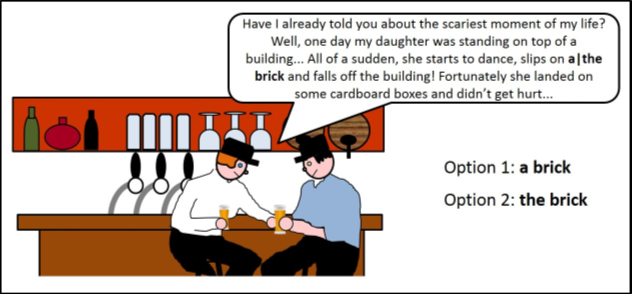
\includegraphics[height=.25\textheight]{figures/fig1.png}
\caption{Example of a non-specific/backgrounded item}
\label{fig:lebruyn:1}
\end{figure}

\begin{figure}[h]
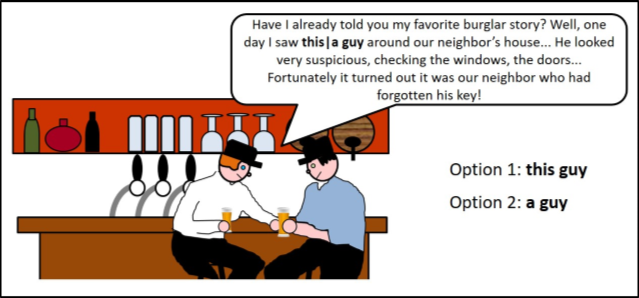
\includegraphics[height=.25\textheight]{figures/fig2.png}
\caption{Example of a specific/backgrounded item}
\label{fig:lebruyn:2}
\end{figure}

The participants were 22 L1 \ili{Mandarin}/L2 \ili{English} speakers. All were undergraduate students of \ili{English} at the Beijing International Studies University. The test was administered by a student assistant in a quiet environment at the university. Participants were tested individually. The instructions as well as the semi-randomized 16 test stories (8 experimental items and 8 fillers) were presented in a PowerPoint presentation with one slide for the instructions and one slide for each test story. Participants were asked to indicate for each story whether they preferred the version with the \is{indefinite articles}indefinite (Option 1) or the \is{definite articles}definite article (Option 2). A small language biography survey was orally carried out by the student assistant to check for the potential influence of stays abroad or other languages. No student had spent time in an \ili{English}-speaking country or mastered another article language than \ili{English}. The participants were given no time limit but all of them completed the experiment in under five minutes.

\tabref{tab:lebruyn:7} summarizes the results of our 22 participants on the test items. L2 learners are at ceiling in the specific/foregrounded condition but produce 31\% of definites in the non-specific/backgrounded condition.

\begin{table}[h]
\begin{tabularx}{.66\textwidth}{XXX}
\lsptoprule
 & \textit{a} & \textit{the} \\
\midrule
Non-specific & 69\% (53/88) & 31\% (27/88)  \\
Specific & 95\% (75/88) & 5\% (5/88) \\
\lspbottomrule
\end{tabularx}
\caption{Percentage of \textit{a} and \textit{the} responses by 22 \ili{Mandarin} respondents in the foregrounded and backgrounded conditions in \citet{LeBruynDong2017T}}
\label{tab:lebruyn:7}
\end{table}
\newpage
To determine the significance of these results, we ran a mixed effects model with item and participant as random factors. There was a significant effect of condition. Pairwise comparisons of the model showed that the foregrounded and the backgrounded conditions were significantly different from each other (t(174)=4.576, p<0.001).

The results indicate that our participants were likelier to produce a definite for non-specific referents than for \is{specificity|)}specific referents. This is exactly the opposite of what we would expect based on the \isi{Fluctuation Hypothesis}. In combination with the data from \citet{Ting2005} and the data we presented in \sectref{sec:lebruyn:4-1}, we conclude that evidence is accumulating that suggests \ili{Mandarin} learners of \ili{English} are different from learners with other article-less L1s in that they do not unequivocally bear out the predictions of the Fluctuation Hypothesis. In \sectref{sec:lebruyn:5}, we propose a research program that aims at establishing L1 influence in article acquisition for learners with an \is{article-less languages}article-less L1. We approach articles as a \is{syntax-semantics interface}syntax/semantics interface phenomenon. The setup of the program allows it to be adapted to study L1 influence for other phenomena at the syntax/semantics interface. 

\section{Establishing L1 influence: A research program}
\label{sec:lebruyn:5}

\citet{Jarvis2000} set the current standard in transfer research. In order to argue for transfer from L1 to L2, he requires a research design with learners from multiple L1 backgrounds that convincingly shows that: (i) learners with the same L1 background pattern together (\textit{intragroup homogeneity}), (ii) learners from different L1 backgrounds behave differently (\textit{intergroup heterogeneity}), and (iii) differences between the groups are linked to differences in their L1s (\textit{cross-linguistic congruity}).

Demonstrating cross-linguistic congruity presupposes cross-linguistic comparison, the study of the many-to-many mapping patterns between the syntax/semantics interfaces (SSIs) of L1s and Target Languages (TLs). For this comparative groundwork, SLA researchers should be able to rely on syntacticians/se\hyp{}manticists. Current work on transfer for articles however shows that the available groundwork will not do. In \sectref{sec:lebruyn:3-1}, we saw that \citet{SnapeLeungTing2006} find that \ili{Mandarin} learners of \ili{English} outperform \ili{Japanese} learners on their acquisition of the \ili{English} \is{articles}article system. They conjecture that this is due to the fact that the \ili{Mandarin} \is{demonstratives}demonstrative \textit{nei} and \is{numeral `one'}numeral \textit{yi} (‘one’) are close to \ili{English} \textit{the} and \textit{a}. If they are right, this entails that the meanings of demonstratives and numerals in \ili{Mandarin} and \ili{Japanese} partly overlap and partly do not and that their relations to demonstratives, numerals and articles in \ili{English} are different. A full argumentation for transfer would then need to focus on those contexts for which \ili{Mandarin} and \ili{Japanese} differ in their use of demonstratives or \isi{numerals}. There is however no work in cross-linguistic syntax/semantics with this level of granularity that transfer research can build on.

The example from \citet{SnapeLeungTing2006} shows us a realistic picture of cross-linguistic syntax/semantics\is{syntax-semantics interface}. Too often, two simplifying assumptions are made: (i) things that superficially look the same are the same (e.g. \isi{numerals}, \isi{demonstratives}), (ii) languages either make the same distinctions or are underspecified (\isi{definiteness}) without there being a (combined) role for other expressions. These simplifications are a limitation in cross-linguistic syntax/semantics. The first challenge a systematic study of L1 influence in article acquisition faces is thus to force a paradigm shift in cross-linguistic syntax/semantics that gives transfer research the groundwork it needs (\textit{the comparative challenge}).

The example from \citet{SnapeLeungTing2006} is also indicative of another challenge the field faces. Transfer research at the SSI is too often synonymous with L2 morpheme studies. This is a reductionist view in two respects. The first is that the SSI is not a mere sum of morphemes but a system in which all morphemes interact. The second is that the SSI of L2 learners can only be properly understood if we model it as a system in which the SSIs of the learner’s L1 and TL come together. We need methodology that allows us to do justice to the full complexity of the SSI of L2 learners (\textit{the L2 interface challenge}). Meeting this challenge allows us to compare the SSIs of L2 learners from the same L1 background and across learner groups (intragroup homogeneity, intergroup heterogeneity) while at the same time comparing them to the L1s and TL of the learners (cross-linguistic congruity).\is{experimental study|)}

\subsection{Iterated Translation Mining}\is{Iterated Translation Mining|(}

Iterated Translation Mining (ITM) overcomes the comparative challenge through the adoption of a data-driven approach in which translation equivalents are used to identify the semantic features that interact with definiteness and study how they are realized cross-linguistically. The output is -- for each language -- an analysis of the SSI of definiteness in the nominal domain. The formalization includes an overview of lexical items/constructions with their associated features (henceforth \textit{feature-based lexicons}) and the rules that govern their use in each of the languages (henceforth \textit{grammars}). To be able to guarantee cross-linguistic comparability, we adopt formal semantics to define the semantic features and we set up the grammars in (Bi-directional) \is{Optimality Theory}Optimality Theory \citep{PrinceSmolensky2004,Hendriksetal2010}. Monolingual reference \is{corpus study|(}corpus and native speaker experiments allow us to overcome the limitations inherent to a corpus-driven approach.
%\newpage
\subsubsection{Data}

ITM uses translation corpora to generate networks of translation equivalents across languages.\footnote{A reviewer correctly points out that the parallel methodology severely restricts the number of languages that can be investigated. We hope this is however only a matter of time in the sense that parallel corpora will hopefully become available for many more languages.} E.g. one takes \textit{a} and \textit{the} as seed words, looks up their uses in the \ili{English} source texts and matches their translations. These can be \isi{demonstratives}, specific word orders, case configurations, etc. As a second step, one looks up all uses of the translations of \textit{a} and \textit{the} in the source and target texts and matches the translations of these in all the languages of the corpus. The first step creates one-way contrastive analyses focusing on how \ili{English} nominal \isi{definiteness} is rendered in the other languages. The second step creates a many-to-many contrastive analysis that gives access to the paradigms of nominal definiteness cross-linguistically with an equal weight for the different languages.

The output of the data collection is a set of contexts with -- for every language -- an indication of the \is{definiteness marking}markers of definiteness. Multi-Dimensional Scaling (MDS) automatically generates clusters of contexts by maximizing the distances between contexts in which (individual) languages use different markers and minimizing the distances between contexts in which the same markers are used (Hamming distance). Based on Analyses of Similarities \citep{Clarke1993,Oksanenetal2017}, we determine the significance of these clusters. The combination of the clusters and the contexts that appear in them is an inductively construed semantic map \citep{Haspelmath1997}, the basis for our cross-linguistic analyses. It furthermore allows us to shift the focus of transfer research from morphemes to the full SSI.

ITM introduces iterations in the Translation Mining technique (TM) we designed with Henriëtte de Swart and Martijn van der Klis \citep{vanderKlisetal2017}.

\subsubsection{Analysis}

The way the analysis proceeds is close to the one in TM \citep[e.g.][]{deSwart2017}. We illustrate with an example in which we apply TM and ITM to the same (hypothetical) dataset. We restrict our attention to two languages (\ili{English} and \ili{Mandarin}) and to a subset of the variation we expect to find.

\begin{figure}[t]
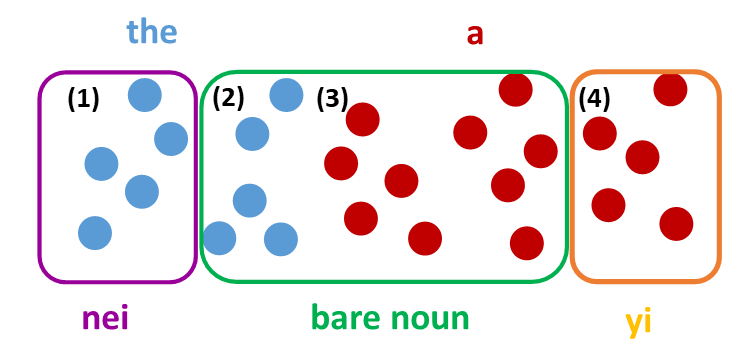
\includegraphics[height=.2\textheight]{figures/TM.png}
\caption{TM}
\label{fig:lebruyn:3}
\end{figure}

\begin{figure}[t]
	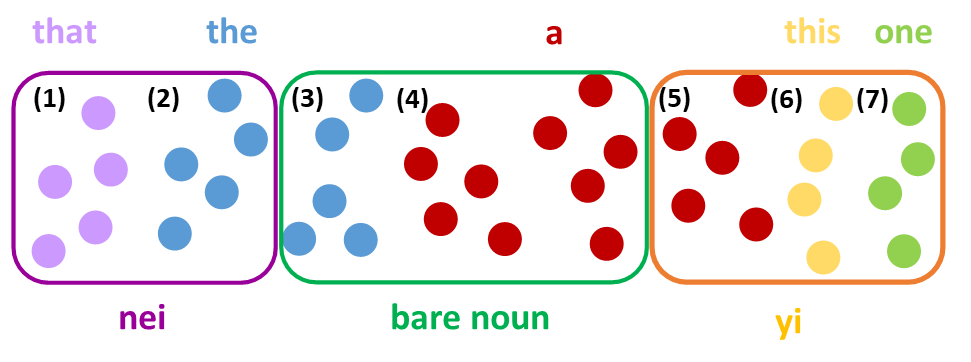
\includegraphics[height=.2\textheight]{figures/ITM.png}
	\caption{ITM}
	\label{fig:lebruyn:4}
\end{figure}

The points in Figures \ref{fig:lebruyn:3} and \ref{fig:lebruyn:4} represent contexts from a translation corpus. Their colours refer to the forms in \ili{English} (upper), the coloured groupings to the forms in \ili{Mandarin} (lower). The clusters that emerge by crossing the form variation in the two languages are numbered.

By inspecting commonalities and differences between clusters, we identify the semantic features at play and the constraints that govern their use. The former are formalized in feature-based lexicons, the latter in bi-directional \is{Optimality Theory}OT grammars. TM presents the picture we know from the literature: \ili{Mandarin} doesn’t have articles and uses \isi{bare nouns} instead with an occasional use of \isi{demonstratives} like \textit{nei} (‘that’) for definites and the \is{numeral `one'}numeral \textit{yi} (‘one’) for \isi{indefinites}. ITM provides the fuller picture we need by translating back the translations of \textit{the} and \textit{a} and providing the relevant oppositions to study the contribution of \textit{the} and \textit{a} when they are not translated by a bare noun and the contribution of \textit{nei} and \textit{yi} when they do function as translations of \textit{the} and \textit{a}. Adding more article-less languages (like \ili{Japanese} and \ili{Russian}) as well as all the iterations allows us to complete this picture (different distribution of bare nouns, demonstratives, \isi{numerals}, case, word order, etc.). The increased complexity is managed through so-called \textit{scenarios} that plot subparts of the data and allow a stepwise analysis of the full picture. The renewed interest in variations of \isi{definiteness} across languages -- not in the least due to Florian Schwarz’s work (\citealt{Schwarz2009,SchwarzToappear}) -- will undoubtedly contribute to the analysis.

\subsection{LOG-IT}

\isi{LOG-IT} (‘Logging Lexicons and \is{Optimality Theory}OT Grammars in Translation’) is a data mining technique that uses a custom-made high quality L1 to L2 translation corpus to inductively study the SSI of individual learners at the same level of detail as the output of ITM. It thus overcomes the L2 interface challenge. 
We use the output of ITM in two ways. The clusters identified through ITM guide our selection of contexts for the translation corpus. For the analysis, we use the ITM feature-based lexicons and OT rules to generate all possible variations on the languages involved. We compare these to the production of the learners and establish individual rankings of these variations. We establish similar rankings for the languages of the project based on our corpus and experimental data. 
The rankings allow us to map and compare the SSI of individual learners, L1 groups and L1/L2s. 

\subsubsection{Data}

We choose written L1 to L2 text translation as a data collection protocol for two reasons:

\begin{enumerate}[(a)]
\item We need data that discriminate between possible rankings. (Semi)-free production tasks cannot target all relevant data per learner.
\item Unlike other high control tasks like Forced Choice Elicitation, translation can focus on any level of production (DP/VP, sentence, \isi{discourse}).
\end{enumerate}


Relying on translation data comes with two risks. The first is a translation bias: learners might be influenced by specific wordings in the source text or resort to general translation processes like simplification. To address this bias, we include two control tasks: a story rewrite task to control for influence from the source text and L2 to L1 translation to control for translation styles. The second risk is overinterpretation of the data: doubts of the learners are not visible in a translation and learners might resort to a word-by-word or sentence-by-sentence strategy while we hope to analyze all levels of production. To address this risk, we exploit the potential of simultaneous key-stroke logging and eye-tracking during translation. We use a combination of measures related to corrections, eye-key spans (\citealt{Timarovaetal2011} and references therein), attention units \citep[e.g.][]{Hvelplund2016}, etc., to establish a measure of reliability per data point. The relevant experimental software goes under the name of TRANSLOG II and was developed in the field of Translation Studies \citep{SchwieterFerreira2017}.

\subsubsection{Analysis}

We use the semantic features and OT grammar constraints identified through ITM to generate all possible lexical entries for the forms used by the learners and all possible \is{Optimality Theory}OT grammars. By crossing lexicons and grammars, we generate all possible variations on the languages involved and rank these per learner. Rankings are based on how accurately the variations predict learner production and \is{corpus study|)}corpus/\is{experimental study}experimental data. Accuracy is established as a measure of (weighted) interrater reliability where the output of the learner and the variation are modeled as raters.

We calculate the distances between learner/language rankings based on the Damerau-Levenshtein distance and establish a dissimilarity matrix. This is the input for Analyses of Similarities that statistically assess intra-group homogene\hyp{}ity/inter-group heterogeneity for the L1 groups. We use MDS to graphically represent similarities and differences between individual learners, learner groups and languages (\figref{fig:lebruyn:5}). In combination with the underlying rankings, the corresponding graph is an inductively constructed map of L1 influence. The underlying data allow us to establish cross-linguistic congruity. 

\begin{figure}\is{LOG-IT}
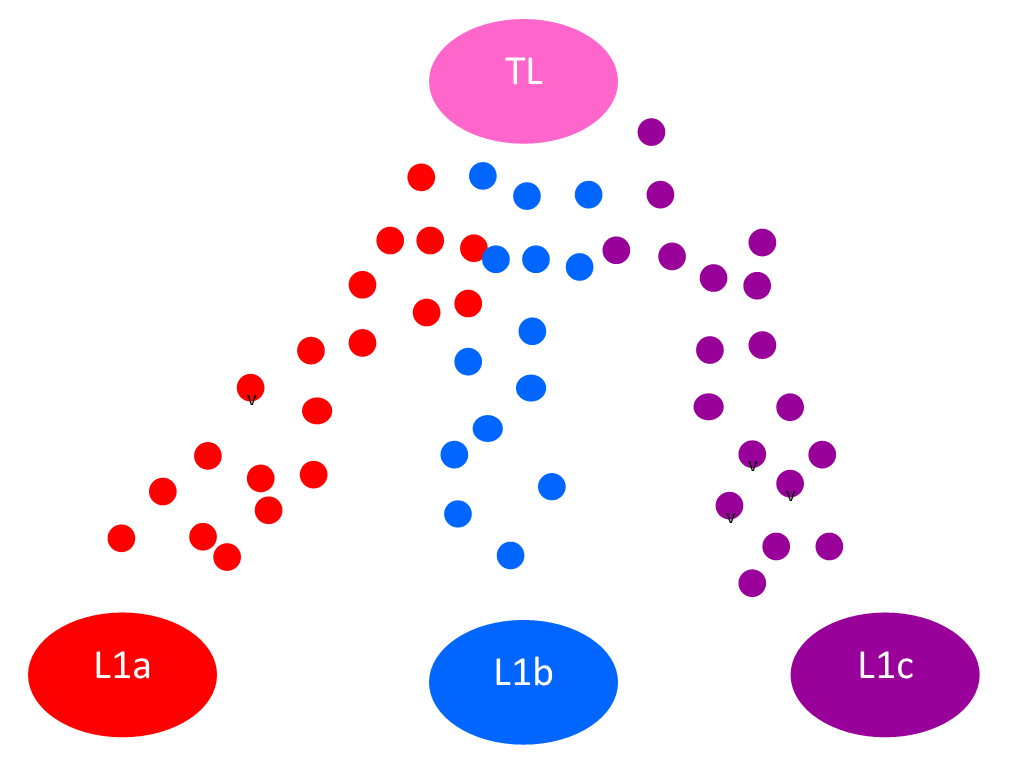
\includegraphics[height=.3\textheight]{figures/LOG-IT.png}
\caption{LOG-IT}
\label{fig:lebruyn:5}
\end{figure}

Characterizing learners in terms of rankings of interlanguages does justice to the variability that characterizes learner languages \citep{LarsenFreeman2006,deBotetal2007}. The logic behind \isi{LOG-IT} allows it to deal with L2s and L3s provided the languages of the learner are included in ITM.\is{Iterated Translation Mining|)}

\section{Conclusion}
\label{lebruyn:6:conclusion}

We have presented evidence suggesting that article-less languages are not created equal and that this influences how native speakers of these languages acquire article languages like \ili{English}. The evidence suggested that \ili{Mandarin} learners of \ili{English} do not unequivocally bear out the predictions of the \isi{Fluctuation Hypothesis}, unlike learners of \ili{English} with e.g. \ili{Korean}, \ili{Russian} and \ili{Japanese} as an L1. 

We have proposed a research program that approaches articles as a \is{syntax-semantics interface}syntax/se\hyp{}mantics interface phenomenon. The program considers the syntax/semantics interface of \isi{definiteness} in its entirety and makes no \textit{a priori} assumptions about how it is best analysed. Rather, it adopts a data-driven comparative approach with multiple L1s that allows us to give a fine-grained answer to the question how L1 influence plays out for definiteness.\is{transfer (from L1 to L2)|)}\is{second language acquisition|)}

%\section*{Abbreviations}
\section*{Acknowledgements}
I would like to thank the editors not only for all their work on the
volume but also for organizing a wonderful conference! Thanks to two
anonymous reviewers for their candid reviews and very useful
suggestions. Special thanks to Xiaoli Dong, Yunhua Hu, Xinyuan Wang,
Zimo Lian and Jordi Martínez. I furthermore gratefully acknowledge the
support of NWO, grant 275-80-006.

{\sloppy
\printbibliography[heading=subbibliography,notkeyword=this]}

\end{document}
